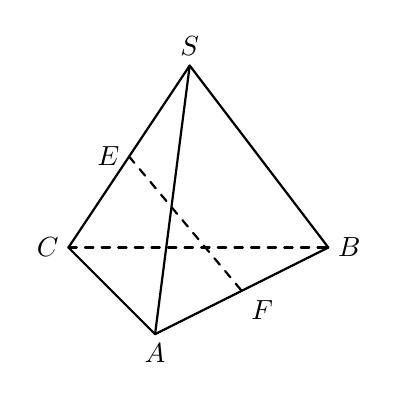
\begin{tikzpicture}[scale=1.1, line cap=round, line join=round]
\usetikzlibrary{calc}
\coordinate (A) at (0,0);
\coordinate (B) at (2,1);
\coordinate (C) at (-1.0,1.0);
\coordinate (S) at (0.4,3.1);

\coordinate (E) at ($(S)!0.5!(C)$);
\coordinate (F) at ($(A)!0.5!(B)$);

\draw[thick] (S)--(A);
\draw[thick] (S)--(B);
\draw[thick] (S)--(C);

\draw[thick] (A)--(B);
\draw[thick] (A)--(C);
\draw[dashed,thick] (C)--(B);

\draw[dashed,thick] (E)--(F);

\node[below] at (A) {$A$};
\node[right] at (B) {$B$};
\node[left]  at (C) {$C$};
\node[above] at (S) {$S$};
\node[left]  at (E) {$E$};
\node[below right] at (F) {$F$};
\end{tikzpicture}